\chapter{Технологическая часть}

\section{Выбор ЯП}

В данной лабораторной работе использовался язык программирования - C\# \cite{Microsoft}.
Данный язык является нативным.
Также я знакома с ним.
Поэтому данный язык был выбран.
В качестве среды разработки я использовала Visual Studio Code \cite{Vs}.
Visual Studio Code подходит не только для  Windows \cite{Win},
но и для Linux \cite{Lin}, это причина,
по которой я выбрала VS code,
т.к. у меня установлена ОС Ubuntu 18.04.4 \cite{Ubuntu}.
В моей архитектуре присутствует 8 ядер.

% Время работы алгоритмов было замерено с помощью класса Stopwatch. Многопоточное программирование было
% реализовано с помощью пространства имен System.Threading.

\section{Сведения о модулях программы}

Данная программа разбита на модули:

\begin{itemize}
	\item Program.cs - Файл, содержащий точку входа в программу.
	\item MainFrom.cs - Файл, содержащий основной код программы.
\end{itemize}

На листингах 3.1-3.4 представлен основной код программы.

\begin{lstlisting}[label=some-code,caption=Метод создания и запуска потоков]
private void DrawScene()
{
	List<Thread> listThread = new List<Thread>();

	int step = 50;
	for (int i = 0; i < (int)SizeObjects.WidthCanvas; i += step)
	{
		listThread.Add(new Thread(new ParameterizedThreadStart(FuncHorizontally)));
		listThread[listThread.Count - 1].Start(new Limit(i, i + step));
	}

	foreach (var elem in listThread)
		elem.Join();

	_imgBox.Image = _img;
}
\end{lstlisting}

\begin{lstlisting}[label=some-code,caption=Метод потока разбиения горизонтально]
public void FuncHorizontally(object obj)
{
	Limit limit = (Limit)obj;
	for (Int32 i = limit.begin; i < limit.end; i++)
		for (Int32 j = 0; j < (int)SizeObjects.HeightCanvas; j++)
			_img.SetPixel(i, j, TraceRay(new Point(i, j)));
}
\end{lstlisting}

\begin{lstlisting}[label=some-code,caption=Метод потока разбиения вертикально]
public void FuncVertically(object obj)
{
	Limit limit = (Limit)obj;
	for (Int32 i = 0; i < (int)SizeObjects.WidthCanvas; i++)
		for (Int32 j = limit.begin; j < limit.end; j++)
			_img.SetPixel(i, j, TraceRay(new Point(i, j)));
}
\end{lstlisting}

\begin{lstlisting}[label=some-code,caption=Однопоточный метод трассировки лучей.]
private void funcTrace()
{
	for (Int32 i = 0; i < (int)SizeObjects.WidthCanvas; i++)
		for (Int32 j = 0; j < (int)SizeObjects.HeightCanvas; j++)
			_img.SetPixel(i, j, TraceRay(new Point(i, j)));
}
\end{lstlisting}

\section{Тестирование}

В данном разделе приведен рис. \ref{ref:res} на котором показан результат работы программы.

\begin{figure}[ht!]
	\centering{
		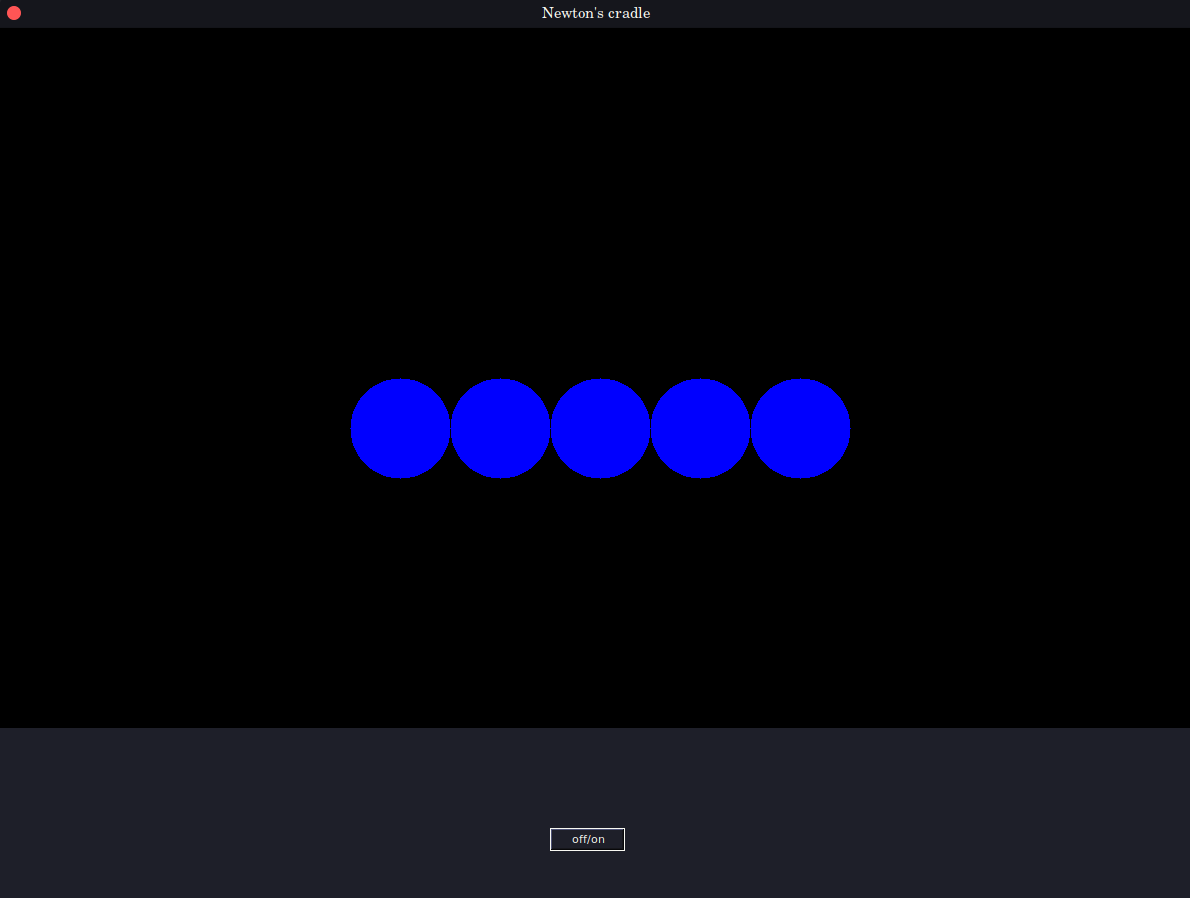
\includegraphics[width=0.8\textwidth]{res.png}
		\caption{Результат работы программы}
		\label{ref:res}}
\end{figure}


\section{Вывод}

В данном разделе были разобраны листинги рис 3.1-3.4, показывающие работу как однопоточного, так и многопоточного
алгоритма трассировки лучей. Также приведен рис. \ref{ref:res}, показывающий корректную работу алгоритма.